\chapter{Descrição da execução do experimento}
	\section{Passo 1 – Desenhar a máquina de estado}
		Com o problema em questão, tem-se em mente que trata-se de uma porta giratória
		que gira no sentido anti-horário.
		Assim, para a elaboração da máquina\footnote{Preferiu-se a utilização de uma máquina de Moore
		por haver conhecimento prévio deste tipo de máquina.}, considerou-se as entradas conforme o
		\autoref{quadro:listaDeEntradas}.

		\begin{quadro}[H]
			\centering
			\caption{Lista das entradas da máquina de estado do problema.}
			\label{quadro:listaDeEntradas}
			\begin{tabular}{|l|l|l|}
			  \hline
			   \textbf{Entrada} & \textbf{Valor lógico 0}  & \textbf{Valor lógico 1}\\
			    \hline
				   Giro & Parado ou sentido horário & Sentido Anti-horário \\
			   	\hline
			   		Entrada & Não há ninguém entrando & Há alguém entrando \\
			    \hline
					Saida & Não há ninguém saindo & Há alguém entrando \\
			    \hline
			    	Metais & Não há metais na entrada & Há metais na entrada \\
			    \hline
			\end{tabular}
			\legend{Fonte: Próprio Autor}
		\end{quadro}

		Com as entradas descritas no \autoref{quadro:listaDeEntradas} elaborou-se a máquina conforme a
		\autoref{figura:maquinaDeEstado}.

		\begin{figure}[H]
			 \centering
			 \caption{\label{figura:maquinaDeEstado}Ilustração da máquina de estado do problema.}
			 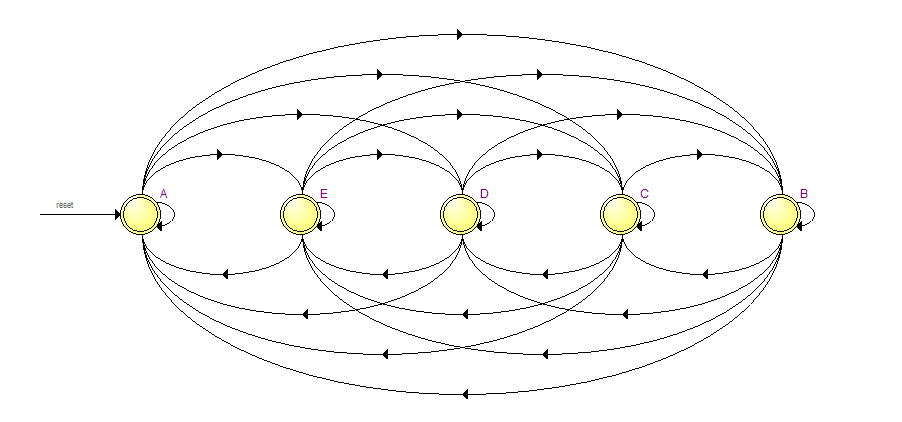
\includegraphics[width=1\textwidth]{img/maquinaDeEstados}
			 \caption*{Nota: A entrada está está descrita na \autoref{figura:tabelaDeTransicao}. O
			  significado dos estados estão no \autoref{quadro:significadoEstados}.}
		\end{figure}

		\begin{figure}[H]
			 \centering
			 \caption{\label{figura:tabelaDeTransicao}Tabela das entradas das transições.}
			 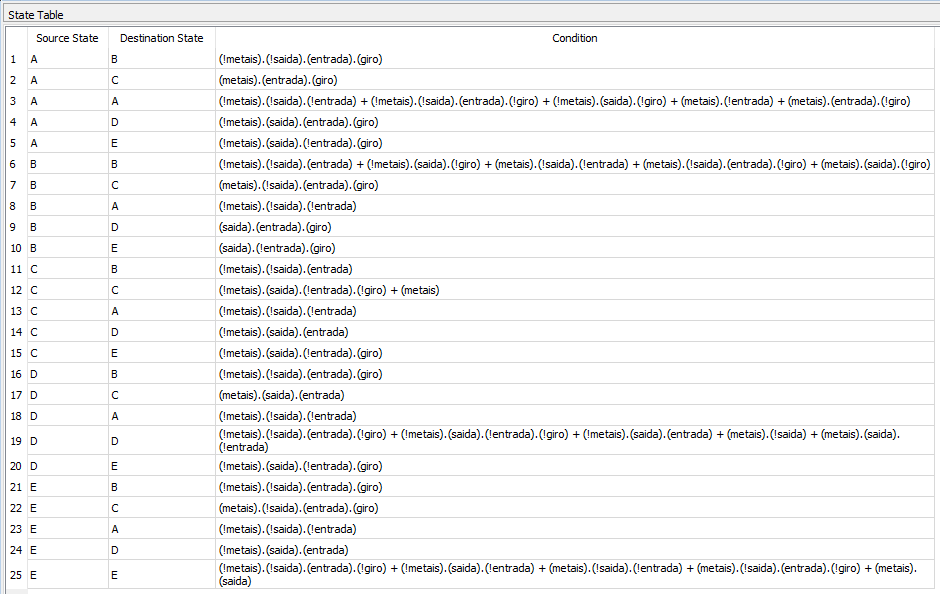
\includegraphics[width=1\textwidth]{img/tabelaDeTransicao}
		\end{figure}

		\begin{quadro}[H]
			\centering
			\caption{Significado dos estados relacionando com os estados reais do problema proposto.}
			\label{quadro:significadoEstados}
			\begin{tabular}{|c|l|}
			  \hline
			   \textbf{Estado} & \textbf{Significado}\\
			    \hline
				   A & Inicial \\
			   	\hline
			   		B & Entrando \\
			    \hline
					C & Detectou metal \\
			    \hline
			    	D & Duas pessoas \\
			    \hline
					E & Saindo \\
				\hline
			\end{tabular}
			\legend{Fonte: Próprio Autor}
		\end{quadro}

	\section{Passo 2 - Escrever um código Verilog para a máquina de estado}
		Para a realização deste passo, foram utilizados o programa Quartus 13.0 SP 1
		 e a placa \ac{fpga} Cyclone II - EP2C20F484C7.

		Com a máquina de estado pronta, criou-se o código em Verilog, que encontra-se no \autoref{codigo:maquina} e o resultado da
		compilação na \autoref{figura:compilacaoMaquina}.

		\lstinputlisting[label = {codigo:maquina},caption = {Código da máquina de estado do problema.}]{codigo/projetoPessoal.v}
		Nota: Para as entradas não mapeadas, a máquina mantêm-se no estado atual.

		\begin{figure}[H]
			 \centering
			 \caption{\label{figura:compilacaoMaquina}Resultado da compilação do código da máquina de
			  estado do problema.}
			 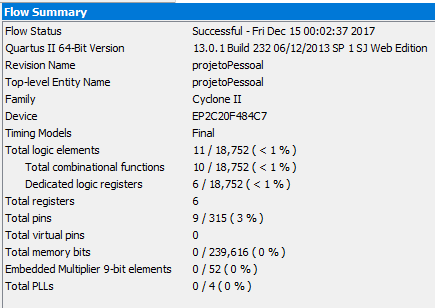
\includegraphics[width=0.7\textwidth]{img/compilacao}
		\end{figure}

		Para a realização dos testes, criou-se um \textit{test bench} conforme o \autoref{codigo:testBenchMaquina}.
		Além disto, fez-se o \textit{deploy} na \ac{fpga}\footnote{Os resultados dos
		 testes e simulações encontram-se na Avaliação dos resultados.}.

		\lstinputlisting[label = {codigo:testBenchMaquina},caption = {Código de \textit{test bench} da máquina do problema.}]
		{codigo/projetoPessoal_TB.v}

%Apresentar   o   detalhamento   da  execução  e   resultados   dos   passos   realizados
%durante   o   experimento,   incluindo   tabelas   verdade,   esquemáticos,   e   código
%(quando  houver).
%Especificar  componentes,  sistemas  e  instrumentos  utilizados.
%Usar listas, figuras e quadros, descrevê-los e discuti-los.



%---------------------------------------------------------------------------------------
